% \documentclass[a5paper,10pt,twoside,openany,article]{memoir}%,draft
\documentclass[a5paper,10pt]{article}
\usepackage[T2A]{fontenc}
\usepackage[utf8x]{inputenc}
\usepackage[english,russian]{babel}
\usepackage{
  % cmap, % copy from pdf
  graphicx,
  subcaption,
  xcolor,
  caption,
  subcaption,
  hyperref, % for url in bibtex
  lineno,
  geometry,
  amssymb,
  amsfonts,
  amsmath, % for \begin{equation*}
  mathtext,
  cite,
  enumerate,
  float, % for figure with [ht]
  calc, % \widthof{999}
  amsthm
}
\usepackage{wrapfig}
\usepackage{tabularx}

\newcommand{\bra}[1]{\left\langle #1 \right|}
\newcommand{\ket}[1]{\left| #1 \right\rangle}
\newcommand{\p}[1]{\left( #1 \right)}
\newcommand{\abs}[1]{\left| #1 \right|}
\newcommand{\tr}[1]{\mathrm{Tr} \left\{ #1 \right\}}
\newcommand{\sx}{I_\mathrm{x}}
\newcommand{\sy}{I_\mathrm{y}}
\newcommand{\sz}{I_\mathrm{z}}
\newcommand{\hdz}{H_\mathrm{dz}}
\newtheorem{definition}{Определение}[section]
\newtheorem{theorem}{Теорема}[section]


\graphicspath{{figures}}
\hypersetup{
  hidelinks, 
  unicode=true  % fix "PD1 encoding, removing `\CYRI'"
} 

% \linenumbers
\geometry{left=15mm,right=15mm,top=20mm,bottom=20mm}
%\captionsetup{font=footnotesize} % smaller caption

\begin{document}
\begin{titlepage}
% \begin{flushright}
%    Приложение № 6 \\
%    к Положению о диссертационном \\
%    совете Московского государственного \\
%    университета имени М.В.Ломоносова
% \end{flushright}
% \vspace{1cm}
\vfill
\begin{center}
  {\large
    Московский государственный университет \\
    имени М.В. Ломоносова
  } \\
  \vfill
  (на правах рукописи) \\
  \vfill
  {\Large \bf Лазарев Илья Дмитриевич} \\
  \vspace{1cm}
  {\Large \bf
      Многочастичная запутанность \\
      в многоквантовой спектроскопии ЯМР \\
      \vspace{2mm}
      в твердом теле
  }
 \vfill
 01.04.07 Физика конденсированного состояния \\
 \vspace{1cm}
 АВТОРЕФЕРАТ \\
 диссертации на соискание ученой степени \\
 кандидата физико-математических наук
 \vfill
 Москва, 2022 г.
\end{center}
\end{titlepage}
\section*{Общая характеристика работы}
\chapter*{Введение}
\addcontentsline{toc}{chapter}{Введение}

% Во введении к диссертации определяется актуальность избранной темы, степень ее разработанности, цели и задачи, объект и предмет исследования, научная новизна, теоретическая и практическая значимость работы, методология диссертационного исследования, положения, выносимые на защиту, степень достоверности и апробация результатов.

% актуальность темы исследования
%   - Квантовые технологии.
%   - Квантовое превосходство.
%   - Квантовая теория информации.
%   - Запутанность в фундаментальных исследованиях.
%   - Квантовые симуляторы и квантовые компьютеры
%
% - степень ее разработанности
%   - История бинарной запутанности
%   - Критерии бинарной запутанности
%   - Эксперименты с бинарной запутанностью
%   - ?? Работы по многочастичной запутанности
%
% - цели и задачи
%   - Разработать теорию МК динамики для системы эквивалентных спинов.
%   - Исследовать многочастичную запутанность в системе эквивалентых спинов.
%   - Исследовать многочастичную запутанность в системе эквивалентных спинов с дипольно упорядоченным начальным состоянием.
%   - Исследовать многочастичную запутанность в одномерной системе.
%   - Разработать экспериментальный метод для определения информации Вигнера-Янасе в МК экcперименте ЯМР.
%   - Провести сравнение результатов оценки многочастичной запутанности на основе информации Вигнера-Янасе и информации Фишера.
%
% - научная новизна
%   - Оценка количества запутанных спинов
%   - Определение информации Вигнера-Янасе
%
% - теоретическую и практическую значимость работы;
%
% - методологию и методы исследования; ??
%
% - положения, выносимые на защиту;
%
% - степень достоверности и апробацию результатов. ??
%
%
% Nowadays, it has been recognized that most physical
% processes in nature can be formulated in terms of processing of information, and information may be central
% to understanding quantum theory [19].
%
%
% проблема классификации и количественной оценки запутанности в целом на сегодняшний день все еще далека от полного понимания.

% Such an investigation of many-spin entanglement is performed for the first time.

\section*{Краткое содержание диссертации}
\textbf{Во введении} дана общая характеристика диссертационной работы,
обоснована актуальность темы,
сформулированы цели работы,
% описана структура диссертации,
показана новизна работы.

\textbf{Первая глава} носит обзорный характер и посвящена роли многочастичной запутанности в квантовой теории информации и методам ее детектирования.
Отмечается, что исследование запутанности между двумя подсистемами хорошо изучено как теоретически, так и экспериментально~\cite{Aldoshin2012}, в отличие от запутанности многих частиц.
В этой главе вводится определение $k$-частично запутанных состояний на основе классификации из работ~\cite{Seevinck2001,Chen2005, Guhne2005}.
Чистое состояние $N$ частиц является $k$-частино запутанным, если
%
\begin{equation}
  \left| \Psi_{k-\mathrm{ent}} \right\rangle
  = \otimes^\mathrm{M}_{i=1} \left| \Psi_{i} \right\rangle,
\end{equation}
%
где $\left| \Psi_{i} \right\rangle$ - это многокубитное несепарабельное или однокубитное состояние подсистемы с $N_i$ частицами
$\left( \sum_{i=1}^N N_i = N \right)$,
и существует такое  $ m \in \mathbb{N}$, что $N_{m} \ge k$.
Смешанное состояние $\rho_{k-\mathrm{ent}}$ может быть представлено как
%
\begin{equation}
  \rho_{k-\mathrm{ent}} =
  \sum\limits_{l} p_l \ket{\Psi_{k_l-\mathrm{ent}}}\bra{\Psi_{k_l-\mathrm{ent}}},
  \end{equation}
%
и существует такое $l$, что $k_l \geq k$.

% Смешанное состояние $\rho_{k-\mathrm{prod}}$
является $k$-разделимым,
если оно может быть факторизовано на $l$ подсистем $\{\rho_i\}$ с размерами $\{N_i\}$,
где $\rho_i$ --- несепарабельное многокубитное состояние или однокубитное состояние,
и выполнено неравенство
\begin{equation}
  N > k \geq N_1 \geq N_2 \geq \dots \geq N_l \geq 1,
  \quad
  \sum_{i=0}^{l} N_i = N.
\end{equation}

Также в этой главе дается обзор методов детектирования многочастичной запутанности.
Особенное внимание уделяется методу оценки количества запутанных частиц в квантовой системе с помощью квантовых информационных величин.
В частности, в этой главе демонстрируется,
что если квантовая информация Фишера системы $N$ частиц с матрицей плотности $\rho$
%
\begin{equation}\label{eq:qfi-entanglement-criteria}
  \qfi(\rho) > \left[ \frac N k \right] k^2 + \p{N - k \left[ \frac N k \right]}^2,
\end{equation}
%
то $\rho$ --- $(k+1)$-частично запутанное состояние~\cite{Hyllus2012}.
Этот результат,
вытекающий из общих свойств квантовой информации,
справедлив~\cite{Chen2005} и для косой информации Вигнера-Янасе.

Так как дальнейшее исследование многочастичной запутанности требует развитие экспериментальных методов,
в этой главе приводится вывод результата, полученного в работе~\cite{Garttner2018},
который открывает возможность экспериментального определения нижней границы квантовой информации Фишера в МК эксперименте ЯМР.

Также в этой главе даются краткий обзор МК эксперимента ЯМР
и примеры образцов, подходящих для исследования многочастичной запутанности в рамках МК спектроскопии ЯМР.


\begin{figure}[H]
  \centering
  \includegraphics[width=0.5\textwidth]{mq-experiment-schema.pdf}
  \caption{\protect\input{figures/mq-experiment-schema}}
  \label{fig:mq-experiment-schema}
\end{figure}


\textbf{Во второй главе} разрабатывается теория МК эксперимента ЯМР для низких температур.
Температура учитывается в начальном термодинамическом равновесном состоянии системы $\rhoEq$,
которое определяется выражением
%
\begin{equation}\label{eq:rho-eq}
  \rhoEq = \rhoEqDefinition,
\end{equation}
%
\rhoEqExplanatoryNote
В данной главе предлагается такое обобщение МК эксперимента ЯМР,
сигнал которого удовлетворяет специальной форме~\cite{Garttner2018} при любых температурах.
Для этого необходимо по прошествии трех периодов МК эксперимента ЯМР (см. Рис.~\ref{fig:mq-experiment-schema}) провести усреднение по начальному состоянию.
В этом случае коррелятор сигнала имеет вид
%
\begin{equation}\label{eq:signal-generalized-short}
  G_\mathrm{LT}(\tau, \phi) = \tr{
   e^{i\phi \sz} \rhoLT (\tau)
   e^{-i\phi \sz} \rhoLT (\tau)
  },
\end{equation}
где $\rhoLT(\tau)$  --- решение уравнения Лиувилля
%
\begin{equation}
  \liouvilleEquation{\hmq}
\end{equation}
%
с начальной матрицей плотности $\rhoEq$~(\ref{eq:rho-eq}).
%
Так как матрицу плотности можно представить~\cite{Feldman1997b}
в виде ряда
\begin{equation}
  \rhoLT (\tau) = \sum_n \rhoLT^{(n)} (\tau),
\end{equation}
%
где $\rhoLT^{(n)}$ вклад в МК когерентность порядка $n$,
учитывая коммутационное соотношение $\commutator{\sz}{\rhoLT(\tau)} = n \rhoLT^{(n)}(\tau)$,
сигнал $G_\mathrm{LT}(\tau, \phi)$ может быть приведен к виду
%
\begin{equation}
  G_\mathrm{LT} = \sum_n e^{in\phi} \tr{
    \rhoLT^{(n)}(\tau)\rhoLT^{(-n)}(\tau)
  }.
\end{equation}
%
Коррелятор сигнала~(\ref{eq:signal-generalized-short}) обобщенного МК эксперимента ЯМР является неупорядоченным по времени коррелятором,
и, следовательно, удвоенный второй момент (дисперсия) $M_2(\tau)$ распределения интенсивностей МК когерентностей ЯМР
является,~\cite{Garttner2018} нижней границей квантовой информации Фишера $F_{Q}$:
%
\begin{equation}\label{eq:qfi-low-bound}
  F_{Q}(\tau)
  \geq 2M_2(\tau)
  = 2 \sum\limits_n n^2 J_\mathrm{LT}^{(n)} (\tau),
\end{equation}
%
где
\begin{equation}\label{eq:coherence-k}
  J_\mathrm{LT}^{(n)} = \tr{\rhoLT^{(n)}(\tau)\rhoLT^{(-n)}(\tau)}.
\end{equation}


\textbf{В третьей главе} исследуется температурная зависимость многочастичной запутанности,
возникающей в нанаполости с большим количеством частиц (\(N\approx50\dots200\)) на подготовительном периоде МК эксперимента ЯМР (см. Рис.~\ref{fig:mq-experiment-schema}).
В качестве модели рассматривается несферическая нанопора, заполненная частицами со спином $\frac 1 2$ (например, ксеноном) в сильном внешнем магнитном поле~\cite{Baugh2001}.
В процессе молекулярной диффузии константа ДДВ усредняется до некоторого ненулевого значения $D_\mathrm{es}$,
которое зависит от формы полости, давления газа и направления сильного внешнего магнитного поля.
По существу нанопора является системой эквивалентных спинов,
и ее МК динамика ЯМР может быть исследована точно.


\begin{figure}[ht]
  \centering
  \begin{subfigure}[t]{0.31\textwidth}
    \centering
    \includegraphics[width=\textwidth]{result-nanopore-eq-m2-by-time-n201-beta0.1.pdf}
    \caption{\protect$\beta=0.1$.
Выше горизонтальной линии детектируется только парная запутанность.
}
    \label{fig:result-nanopore-eq-m2-by-time-beta0.1}
  \end{subfigure}
  \hfill
  \begin{subfigure}[t]{0.32\textwidth}
    \centering
    \includegraphics[width=\textwidth]{result-nanopore-eq-m2-by-time-n201-beta0.5.pdf}
    \caption{\protect$\beta=0.5$.
В полосе, ограниченной горизонтальными линиями ($k=14$ и $k=27$),
детектируется запутанность от 15 до 27 спинов.}
    \label{fig:result-nanopore-eq-m2-by-time-beta0.5}
  \end{subfigure}
  % \hfill
  % \begin{subfigure}[t]{0.45\textwidth}
  %   \centering
  %   \includegraphics[width=\textwidth]{result-nanopore-eq-m2-by-time-beta1.pdf}
  %   \caption{\protect\input{figures/result-nanopore-eq-m2-by-time-beta1}}
  %   \label{fig:result-nanopore-eq-m2-by-time-beta1}
  % \end{subfigure}
  \hfill
  \begin{subfigure}[t]{0.34\textwidth}
    \centering
    \includegraphics[width=\textwidth]{result-nanopore-eq-m2-by-time-n201-beta3.5.pdf}
    \caption{\protect$\beta=3.5$.
Детектируется запутанность почти всех спинов ($179$ из $201$).
}
    \label{fig:result-nanopore-eq-m2-by-time-beta3.5}
  \end{subfigure}
  \caption{\protect Зависимость нижней границы квантовой информации Фишера $F_Q = 2M_2(\tau)$ от безразмерного времени $D_\mathrm{es}\tau$ с термодинамическим равновесным начальным состоянием $\rhoEq$ системы с $N=201$ частиц.
 % Горизонтальные линии соответствуют максимальным значениям информации Фишера $k$-разделимых состояний.
}
  \label{fig:result-nanopore-eq-m2-by-time-betas}
\end{figure}

На подготовительном периоде МК эксперимента ЯМР гамильтониан системы эквивалентных спинов определяется выражением
%
\begin{equation}\label{eq:mq-hamiltoninan-equivalent-spins}
  \hmqEquivalentSpinsDefinition
\end{equation}
%
\hmqEquivalentSpinsExplanatoryNote
Так как гамильтониан~$\hmqEquivalentSpins$ коммутирует с квадратом полного спинового углового момента $\soperator^2$ ($\commutator{\hmqEquivalentSpins}{\soperator^2} = 0$),
он может быть разбит на блоки $\hmqEquivalentSpins^S$,
соответствующие различным значениям $S$ полного спинового углового момента
%
\begin{equation}\label{eq:total-angular-momentum-values}
  \totalSpinAnglularMomentumValuesDefinition,
\end{equation}
%
\totalSpinAnglularMomentumValuesExplanatoryNote
Когда начальное состояние системы $\rho(0)$ тоже коммутирует с квадратом полного спинового углового момента $\soperator^2$ ($\commutator{\rho(0)}{\soperator^2} = 0$),
можно перейти к рассмотрению динамики отдельных блоков $\rho^S(0)$, размер которых равен $2S+1$,
а степень вырождения $\hmqEquivaletnSpinsBlockDegeneration$ равна~\cite{Landau3}
%
\begin{equation}
  \hmqEquivaletnSpinsBlockDegenerationDefinition.
\end{equation}
В этом случае выражение для МК когерентности, наблюдаемой в обобщенном МК эксперименте ЯМР, может быть записано в виде
%
\begin{equation}\label{eq:coherence_k}
  J^{(n)}(\tau) = \sum_S \hmqEquivaletnSpinsBlockDegeneration J^{(n), S}(\tau),
  \quad
  (-N \leq n \leq N),
\end{equation}
%
где
\begin{equation}\label{eq:coherence_k_block}
  J^{(n), S} = \tr{\rho^{(n), S}(\tau)\rho^{(-n), S}(\tau)},
\end{equation}
а $\rho^{(n), S}(\tau)$ --- эволюционная матрица плотности соответсвующая блоку $S$.

\begin{wrapfigure}{O}{0.4\textwidth}
  \includegraphics[width=0.4\textwidth]{result-nanopore-eq-nent-by-beta.pdf}
  \caption{\protectЗависимость максимального задетектированного размера запутанного кластера от обратной температуры
$\beta = \frac{\hbar\omega_0}{kT} $}
  \label{fig:result-nanopore-eq-nent-by-beta}
\end{wrapfigure}

Термодинамическая равновесная матрица плотности $\rhoEq$,
определенная в выражении~(\ref{eq:rho-eq}),
коммутирует с квадратом полного углового момента
($\commutator{\rhoEq}{\soperator^2} = 0$).
Поскольку гамильтониан $\hmqEquivalentSpins$ и матрица плотности в начальный момент времени $\rho(0) = \rhoEq$ могут быть приведены к блочно диагональному виду,
можно численно рассчитать эволюцию каждого блока $\rhoEq^S$.
Так как гамильтониан $\hmqEquivalentSpins$ не зависит от времени,
уравнение Лиувилля для блока $\rhoLT^S(\tau)$ эволюционной матрицы плотности имеет вид
%
\begin{equation}\label{eq:rho_block_eval_lt}
  \rhoLT^S(\tau) = e^{-i \hmqEquivalentSpins^S \tau}
    \rhoEq^S e^{i \hmqEquivalentSpins^S \tau}.
\end{equation}
%
Подставляя выражение~(\ref{eq:rho_block_eval_lt})  в~(\ref{eq:coherence_k_block}) и~(\ref{eq:coherence_k}), получаем интенсивности МК когерентностей ЯМР,
второй момент распределения которых определяет~(\ref{eq:qfi-low-bound}) нижнюю границу информации Фишера.

В этой главе диссертации приводится аналитическое решение для системы из $N=3$ частиц.
В этом случае возникают когерентности только нулевого и плюс/минус второго порядков.
Полученные выражения для нормированных интенсивностей имеют вид
%
\begin{align}\label{eq:j_lt_3}
  J_{\mathrm{LT}, 0}(\tau) & = 1 - \frac 1 2 \tanh^2(\beta)\sin^2\p{\sqrt 3 D_\mathrm{es} \tau}, \\
  J_{\mathrm{LT},\pm 2}(\tau) & = \frac 1 4 \tanh^2(\beta)\sin^2\p{\sqrt 3 D_\mathrm{es} \tau}.
\end{align}


Результаты численных расчетов зависимости нижней границы информации Фишера от времени для системы с $N=201$ частиц приведены на Рис.~\ref{fig:result-nanopore-eq-m2-by-time-betas}.

На Рис.~\ref{fig:result-nanopore-eq-m2-by-time-beta0.1} значение параметра $\beta = 0.1$ соответствует температуре ${T= 2.4\cdot 10^{-1}}$~K при ларморовской частоте $\omega_0 = 2\pi\cdot 500\cdot10^6$ с$^{-1}$.
Неравенство~(\ref{eq:qfi-entanglement-criteria}) может быть выполнено только при $k=1$ (горизонтальная линия на Рис.~\ref{fig:result-nanopore-eq-m2-by-time-beta0.1}).
Это подтверждает, что в высокотемпературном случае возможна парная запутанность~\cite{Feldman2012}.

При температуре $T = {4.8\cdot10^{-2}}$~K $(\beta=0.5)$ на Рис.~\ref{fig:result-nanopore-eq-m2-by-time-beta0.5} видна полоса, в которой неравенство~(\ref{eq:qfi-entanglement-criteria}) может быть удовлетворено, когда $14 \leq k < 27$.

При понижении температуры ширина полосы, где детектируется многочастичная запутанность, увеличивается.
При температуре $T= 6.856\cdot10^{-3}$~K $(\beta=3.5)$
почти все спины (до 179 из 201) запутаны (см. Рис.~\ref{fig:result-nanopore-eq-m2-by-time-beta3.5}).
Запутанность существует в течение всего процесса эволюции, за исключением короткого начального периода времени.

На Рис.\ref{fig:result-nanopore-eq-nent-by-beta} точками представлено максимальное значение запутанности за период ($0 \leq D_\mathrm{es}\tau \leq 10$) при различных значениях обратной температуры $\beta$.
Количество запутанных спинов увеличивается при понижении температуры.

Многочастичную запутанность также можно исследовать,
когда та же самая система первоначально приготовлена в дипольном упорядоченном состоянии~\cite{Goldman1970}.
В работе~\cite{Doronin2011} отмечается,
что в этом случае МК~когерентности~ЯМР~возникают быстрее.

\begin{figure}[H]
  \centering
  \begin{subfigure}[t]{0.3\textwidth}
    \centering
    \includegraphics[width=\textwidth]{figures/result-nanopore-do-m2-by-time-n101-beta1.png}
    \caption{\protect$T=6\cdot10^{-4}$~K.
Выше горизонтальной линии детектируется только парная запутанность.
}
    \label{fig:result-nanopore-do-m2-by-time-n101-beta1}
  \end{subfigure}
  \hfill
  \begin{subfigure}[t]{0.3\textwidth}
    \centering
    \includegraphics[width=\textwidth]{figures/result-nanopore-do-m2-by-time-n101-beta2.png}
    \caption{\protect\input{figures/result-nanopore-do-m2-by-time-n101-beta2}}
    \label{fig:result-nanopore-do-m2-by-time-n101-beta2}
  \end{subfigure}
  \hfill
  \begin{subfigure}[t]{0.3\textwidth}
    \centering
    \includegraphics[width=\textwidth]{figures/result-nanopore-do-m2-by-time-n101-beta3.png}
    \caption{\protect\input{figures/result-nanopore-do-m2-by-time-n101-beta3}}
    \label{fig:result-nanopore-do-m2-by-time-n101-beta3}
  \end{subfigure}
  \caption{\protectЗависимость нижней границы квантовой информации Фишера $F_Q = 2M_2(\tau)$ от безразмерного времени $D_\mathrm{es}\tau$ с дипольным упорядоченным начальным состоянием $\rhoDo$ системы с $N=101$ частиц.
% Горизонтальные линии соответствуют максимальным значениям информации Фишера $k$-разделимых состояний.}
  \label{fig:result-nanopore-do-m2-by-time-n101-betas}
\end{figure}

В общем случае в начальный момент времени система находится в термодинамическом равновесии с матрицей плотности
%
\begin{equation}\label{eq:rho-eq-hdz}
  \rho(0) = \rhoEqHdz = \rhoEqHdzDefinition,
\end{equation}
\rhoEqHdzExplanatoryNote
%
Используя  метод адиабатического размагничивания во вращающейся системе координат (ВСК)~\cite{Goldman1970, Slichter1961}
либо двухимпульную последовательность Брокаерта-Джинера,
можно получить систему в состоянии термодинамического равновесия с матрицей плотности
%
\begin{equation}\label{eq:do-state}
 \rhoDo = \rhoDoDefinition,
\end{equation}
\rhoDoExplanatoryNote

Магнитное упорядочение~\cite{Abragam1982} выходит за рамки диссертации,
и рассматривается только промежуточный температурный случай,
когда зеемановская температура является низкой $({\frac{\hslash \omega_{0}}{k} \alpha_\mathrm{z}}\gg 1)$,
а дипольная --- высокой $\p{ \frac{\hslash{D}}{k}\beta_\mathrm{d} \ll 1}$.
Тогда выражение~(\ref{eq:do-state}) матрицы плотности~$\rho_i$ может быть разложено в ряд по $\beta_\mathrm{d}$:
%
\begin{equation}\label{eq:do-state-ht}
  \rhoDo \approx \rhoDoDefinitionHT.
\end{equation}
%
В оригинальной работе~\cite{Jeener1967} двухимпульсный эксперимент Брокаерта-Джинера был разработан для высокотемпературного случая.
В этой главе диссертации теоретически показано,
что этот эксперимент также может выполняться и для промежуточного температурного случая.

В нанопоре гамильтониан $\hdz$ частично усредняется за счет быстрой молекулярной диффузии
и может быть записан~\cite{Feldman2004,Doronin2011} в виде
%
\begin{equation}\label{eq:hdz-mean}
  \hdzEquivaletnSpins = \hdzEquivaletnSpinsDefinition,
\end{equation}
\hdzEquivaletnSpinsExplanatoryNote
%
Таким образом, начальное состояние $\rhoDo$~(\ref{eq:do-state-ht}) может быть разделено на блоки $\rhoDo^S$, соответствующие различным значениям $S$~(\ref{eq:total-angular-momentum-values}) полного спинового углового момента.
Эволюция блока $\rhoDo^S$ определяется уравнением Лиувилля
%
\begin{equation}\label{eq:rho-block-eval-do}
  \rhoDo^S(\tau) = e^{-i \hmqEquivalentSpins^S \tau}
    \rhoDo^S e^{i \hmqEquivalentSpins^S \tau}.
\end{equation}
%
Подставляя выражение~(\ref{eq:rho-block-eval-do})  в~(\ref{eq:coherence_k_block}) и~(\ref{eq:coherence_k}), получаем интенсивности МК когерентностей ЯМР.

В этой главе диссертации приводится аналитическое решения для системы из $N=3$ частиц.
В такой системе возникают когерентности только нулевого и плюс/минус второго порядков.
Полученные выражение для нормированных интенсивностей имеют вид
%
\begin{align}\label{eq:coherences-n3-do}
    J_{\mathrm{do}, 0}(\tau) & = 1
    - \dfrac 1 2 \tanh^2\p{ \dfrac{3 \beta^* }{2} }
      \sin^2 \p{ \sqrt{3} D\tau },
    \\
    J_{\mathrm{do},\pm2}(\tau) & = \dfrac{1}{4}
      \tanh^2 \p{ \dfrac{3 \beta^*}{2} }
      \sin^2 \p{ \sqrt{3} Dt },
\end{align}
где $\beta^* = {\frac{\hslash}{k} \beta_\mathrm{d} D_\mathrm{es}}$.

Результаты численных расчетов зависимости нижней границы информации Фишера~(\ref{eq:qfi-low-bound}) от времени для системы с $N=101$ частиц приведены на Рис.~\ref{fig:result-nanopore-do-m2-by-time-n101-betas}.
Из Рис.~\ref{fig:result-nanopore-do-m2-by-time-n101-beta1} видно,
что при температуре $T=6\cdot10^{-4}$~K детектируется только парная запутанность.
При температуре $T=3.2\cdot10^{-4}$~K на Рис.~\ref{fig:result-nanopore-do-m2-by-time-n101-beta2} появляется полоса, в которой неравенство~(\ref{eq:qfi-entanglement-criteria}) может быть выполнено, когда $19 \leq k < 46$.
Таким образом, детектируется многочастичная запутанность от 20 до 46 спинов.
Когда температура понижается, ширина полосы, в которой существует многочастичная запутанность, увеличивается.
При температуре $T=4.8\cdot10^{-5}$~K (Рис.~\ref{fig:result-nanopore-do-m2-by-time-n101-beta3}) детектируется запутанность почти всех спинов (92 из 101).

\begin{figure}[H]
 	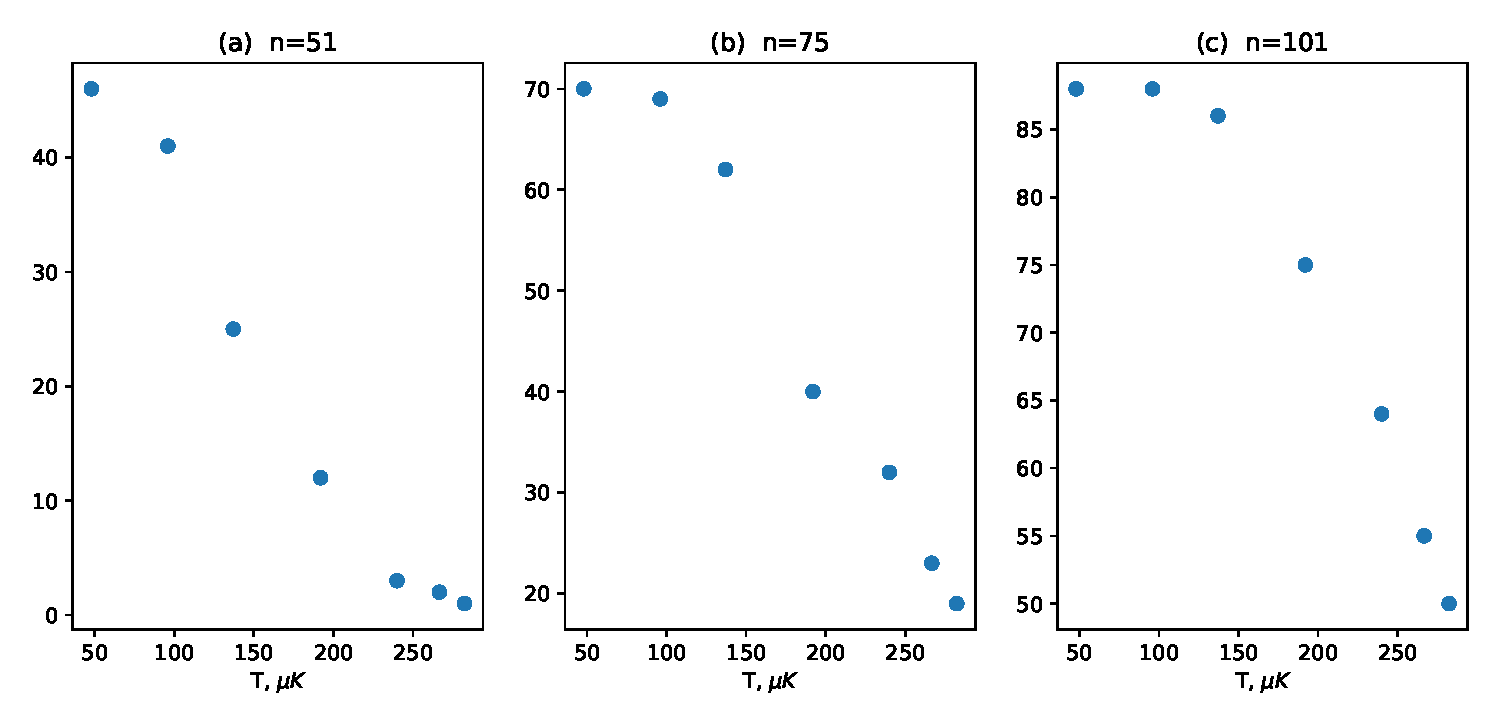
\includegraphics[width=\textwidth]{result-nanopore-do-nent-by-beta-n51-n75-n101.eps}
	\caption{\protectЗависимость максимального задетектированного размера запутанного кластера
за интервал времени эволюции $(0 \leq D\tau \leq 3)$,
от температуры при  a) $N=51$; b) $N=75$; c) $N=101$.
}
	\label{fig:result-nanopore-do-nent-by-beta-n51-n75-n101}
\end{figure}

Зависимость максимального размера запутанного кластера за время эволюции $({0}\leq \mathrm{D}\tau\leq{3})$ от температуры при разных числах спинов в нанопоре представлена на Рис.~\ref{fig:result-nanopore-do-nent-by-beta-n51-n75-n101}.
Максимальное количество запутанных спинов уменьшается при повышении температуры.
Максимальное количество запутанных спинов увеличивается, когда увеличивается число спинов в нанопоре, потому что система в нанопоре становится плотнее.


\textbf{В четвертой главе} исследуется многочастичная запутанность в цепочках ядерных спинов.

\begin{wrapfigure}{O}{0.3\textwidth}
  \includegraphics[width=0.3\textwidth]{model-zchain-schema}
  \caption{\protectСхема зигзагообразной цепочки ядерных спинов.
Нечетные звенья параллельны внешнему магнитному полю $\vec{H}_0$,
а $\varphi$ --- угол между соседними звеньями.
% Константы связи $D_1$ и $D_2$ определяются уравнением~(\ref{eq:dipolaconstantsnearest}), а $D_3=D_{n, n+2},\, (n=1,2,...)$
% уравнением~(\ref{eq:dipolaconstantsnextnearest}).
}
  \label{fig:model-zchain-schema}
\end{wrapfigure}

Однородная цепочка является наиболее простой и хорошо изученной разновидностью одномерной системы.
Создание запутанных кластеров в таких цепочках ограничено слабыми ДДВ удаленных спинов.
В МК эксперименте ЯМР в однородной цепочке существенны только когерентности нулевого и плюс/минус второго порядков. Неравенство~(\ref{eq:qfi-entanglement-criteria}) выполняется только для $k = 1$, то есть детектируется только парная запутанность.
Полученная оценка согласуется с представленными в литературе~\cite{Doronin2007, Feldman2012} результатами.
% Также в этой главе отмечается, что увеличение длины цепочки
% не всегда ведет к увеличению числа запутанных спинов.
Этого достаточно для передачи МК когерентностей вдоль цепочки~\cite{Bochkin2018qip, Feldman2021, Zhukov2019, Bochkin2022} и создания запутанности между удаленными концами цепочки~\cite{Lazarev2019}.
В однородных цепочках константа ДДВ ближайших соседей
в восемь раз превышает константу ДДВ следующих ближайших соседей. В зигзагообразных цепочках
роль следующих ближайших соседей является более существенной, что ведет к необходимости учитывать
МК когерентности четвертого порядка~\cite{Bochkin2019}.
% Данное обстоятельство является важным для исследования многочастичной запутанности,
% поскольку при этом используется второй момент распределения МК когерентностей ЯМР.


На Рис.~\ref{fig:model-zchain-schema} схематично представлена
зигзагообразная цепочка ядерных спинов в сильном внешнем магнитном поле $\vec{H}_0$.
Нечетные звенья цепочки параллельны внешнему магнитному полю $\vec{H}_0$,
а $\varphi$ --- угол между соседними звеньями.
Гамильтониан,
описывающий МК динамику ЯМР зигзагобразной цепочки с учетом взаимодействия со следующими ближайшими соседями, задается выражением~\cite{Doronin2000}
%
\begin{equation}\label{hmq-next-nearest}
  \hmqZChainNextNearest = \hmqZChainNextNearestDefinition,
\end{equation}
%
\hmqZChainNextNearestExplanatoryNote
%
Константы ДДВ
в зигзагообразной цепочке определяются выражениями~\cite{Abragam1982}
%
\begin{align}\label{eq:dipolar-constants-nearest}
  D_{2n-1, 2n} & = D_1 =\dfrac{\gamma^2\hbar }{r^3},
  \\
  D_{2n, 2n+1} & = D_2=\dfrac{\gamma^2\hbar }{2r^3}\p{3\cos^2 \varphi -1},
  \quad n=1,2\dots,
\end{align}
%
где $\gamma$ --- гиромагнитное отношение,
$r$ --- расстояние между ближайшими спинами в цепочке.
Также в гамильтониане учитываются взаимодействия со следующими соседями,
константа диполь-дипольного взаимодействия которых определяется как~\cite{Abragam1982}
%
\begin{equation}\label{eq:dipolaconstantsnextnearest}
  D_{n, n+2}=\dfrac{\gamma^2\hbar }{16r^3 \sin^3 \frac{\varphi}{2}}\p{3\sin^2 \frac{\varphi}{2} -1}.
\end{equation}
%
В частности, уравнения~(\ref{eq:dipolar-constants-nearest}),~(\ref{eq:dipolaconstantsnextnearest}) означают,
что для прямой спиновой цепочки, когда  $(\varphi=\pi)$,
константа дипольной связи для ближайших соседей в восемь раз больше,
чем константа дипольной связи между следующими ближайшими соседями.
При $\varphi=\frac{2\pi}{3}$ отношение констант связи
\begin{equation}
  \left|\dfrac{D_{2n, 2n+1}}{D_{2n-1, 2n+1}}\right| = \dfrac{3\sqrt{3}}{5}.
\end{equation}
Следовательно, ДДВ следующих ближайших соседей
существенны для МК динамики ЯМР при определённых ориентациях зигзагообразной спиновой цепочки
по отношению к направлению внешнего сильного магнитного поля.

\begin{figure}[ht]
  \begin{subfigure}[t]{0.32\textwidth}
    
\includegraphics[width=\textwidth]{result-zchain-m2-by-time-n6-beta10}
    \caption{\protect$\beta=10$ ($T = 2.4\times 10^{-3}$~К), $N=6$.
В области выше горизонтальной линии $k=1$ детектируется парная запутанность, выше $k=5$ --- шестиспиновая запутанность.
}
    \label{fig:result-zchain-m2-by-time-n6-beta10}
  \end{subfigure}
  \hfill
  \begin{subfigure}[t]{0.32\textwidth}
    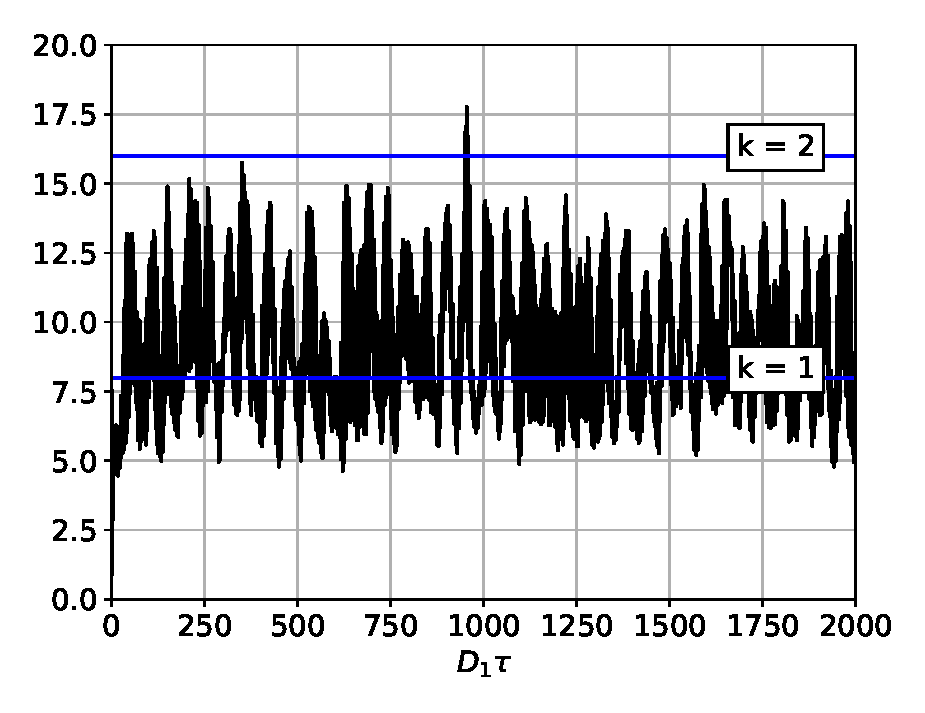
\includegraphics[width=\textwidth]{result-zchain-m2-by-time-n8-beta1}
    \caption{\protect$\beta = 1$ ($T = 2.4\times 10^{-2}$~К), $N=8$.
В области ограниченной горизонтальными линиями $k=1$ и $k=2$
детектируется парная запутанность.
}
    \label{fig:result-zchain-m2-by-time-n8-beta1}
  \end{subfigure}
  \hfill
  \begin{subfigure}[t]{0.32\textwidth}
    
\includegraphics[width=\textwidth]{result-zchain-m2-by-time-n8-beta20}
    \caption{\protect$\beta = 20$ ($T = 1.2\times 10^{-3}$~К), $N=8$.
В области ограниченной горизонтальными линиями $k=2$ и $k=4$
детектируется трехчастичная запутанность.
}
    \label{fig:result-zchain-m2-by-time-n8-beta20}
  \end{subfigure}
  \caption{\protectЗависимость нижней границы квантовой информации Фишера~$F_Q=2M_2(\tau, \beta)$
от безразмерного времени~$D_1\tau$
в зигзагообразной цепочке.
% Горизонтальные линии соответствуют максимальным значениям информации Фишера $k$-разделимых состояний.}
  \label{fig:result-zchain-m2-by-time-ns-betas}
\end{figure}

% \begin{wrapfigure}{O}{0.5\textwidth}
%   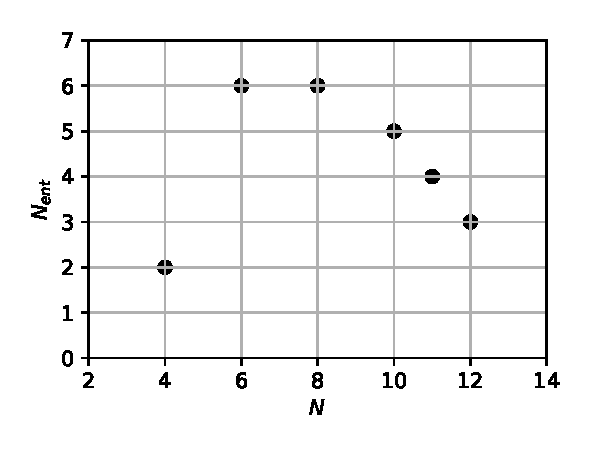
\includegraphics[width=0.5\textwidth]{result-zchain-nent-by-n-beta10}
%   \caption{\protectЗависимость максимального задетектированного размера запутанного кластера~$N_{ent}$ от длины цепочки $N$ при температуре $\beta = 10$ ($T = 2.4\times 10^{-3}$~К).
}
%   \label{fig:result-zchain-nent-by-n-beta10}
% \end{wrapfigure}

Эволюционная матрица плотности зигзагобразной цепочки на подготовительном периоде МК эксперимента ЯМР (Рис.~\ref{fig:mq-experiment-schema})
с термодинамическим начальным состоянием $\rhoEq$
определяется выражением
%
\begin{equation}\label{eq:rho-eval-zchain}
  \rho_\mathrm{zc}(\tau) = e^{-i \hmqZChainNextNearest \tau}
    \rhoEq e^{i \hmqZChainNextNearest \tau}.
\end{equation}
%
Интенсивности  МК когерентностей ЯМР определяются уравнением~(\ref{eq:coherence-k}),
а нижняя граница информации Фишера --- из выражения~(\ref{eq:qfi-low-bound}).
При обратной температуре $\beta=0.5$,
что соответствует температуре $T=4.8 \times 10^{-2}\,\mbox{K}$
при ларморовской частоте $\omega_0=2\pi\times 500\times 10^6 \,\mbox{s}^{-1}$,
для спиновых цепочек с $N=6$ и $N=8$
неравенство~(\ref{eq:qfi-entanglement-criteria})  выполняется только при $k=1$.
Это означает, что в высокотемпературном случае
детектируется только парная запутанность,
что согласуется с работой~\cite{Feldman2012}.

% \begin{wrapfigure}{O}{0.5\textwidth}
%   \centering
%   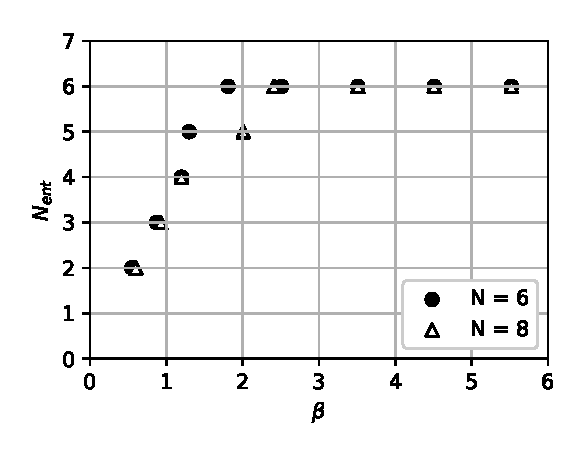
\includegraphics[width=0.5\textwidth]{result-zchain-nent-by-beta-n8-n6}
%   \caption{\protectЗависимость максимального задетектированного размера запутанного кластера~$N_{ent}$ от обратной температуры $\beta$
в зигзагообразной цепочке,
состоящей из шести и восьми спинов.}
%   \label{fig:result-zchain-nent-by-beta-n8-n6}
% \end{wrapfigure}


Временная эволюция нижней границы квантовой информации Фишера,
соответствующая  удвоенному второму моменту распределения интенсивностей МК когерентностей~(\ref{eq:qfi-low-bound}) для шестиспиновой цепочки, представлена на Рис.~\ref{fig:result-zchain-m2-by-time-n6-beta10} при температуре $T = 2.4\times 10^{-3}\,\mbox{K}$ $(b=10)$.
На Рис.~\ref{fig:result-zchain-m2-by-time-n6-beta10} видна полоса,
в которой неравенство~(\ref{eq:qfi-entanglement-criteria}) удовлетворено при $1\leqslant k \leqslant 5$.
Таким образом, детектируется многочастичная запутанность в спиновых кластерах, состоящих из 2-6 спинов.
Зависимость максимального размера запутанного кластера от длины цепи приведена на Рис.~\ref{fig:result-zchain-nent-by-n-beta10} при температуре $T = 2.4\times 10^{-3}\,\mbox{K}$.

Временная эволюция нижней границы информации Фишера в восьмиспиновой зигзагообразной цепочке представлена на Рис.~\ref{fig:result-zchain-m2-by-time-n8-beta1}
и Рис.~\ref{fig:result-zchain-m2-by-time-n8-beta20}.
При температуре $T=2.4\times 10^{-2}$~К возникают многочастичные запутанные кластеры,
состоящие из двух или трех спинов,
а при температуре $T=1.2\times 10^{-2}$~К возникают запутанные кластеры размером от 2 до 4 спинов.


\begin{figure}[H]
  \begin{subfigure}[t]{0.48\textwidth}
    \centering
    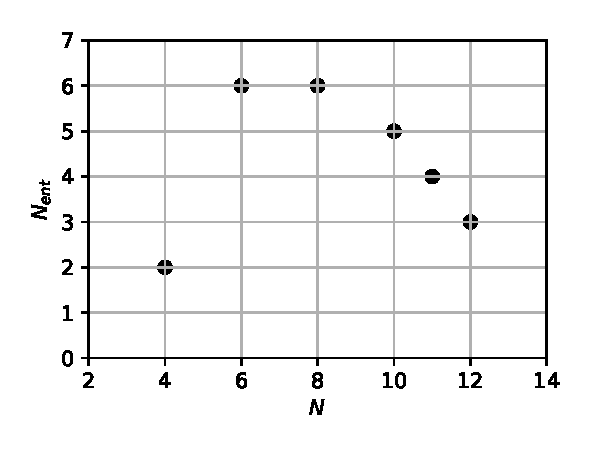
\includegraphics[width=\textwidth]{result-zchain-nent-by-n-beta10}
    \caption{}
    % \caption{\protectЗависимость максимального задетектированного размера запутанного кластера~$N_{ent}$ от длины цепочки $N$ при температуре $\beta = 10$ ($T = 2.4\times 10^{-3}$~К).
}
    \label{fig:result-zchain-nent-by-n-beta10}
  \end{subfigure}
  \hfill
  \begin{subfigure}[t]{0.48\textwidth}
    \centering
    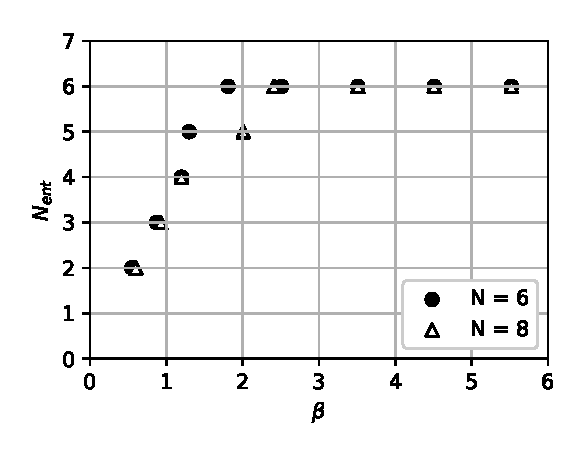
\includegraphics[width=\textwidth]{result-zchain-nent-by-beta-n8-n6}
    \caption{}
    % \caption{\protectЗависимость максимального задетектированного размера запутанного кластера~$N_{ent}$ от обратной температуры $\beta$
в зигзагообразной цепочке,
состоящей из шести и восьми спинов.}
    \label{fig:result-zchain-nent-by-beta-n8-n6}
  \end{subfigure}
  \label{fig:result-zchain-nent-by-betaand-n}
  \caption{\protect Зависимость максимального числа запутанных спинов~$N_{ent}$ от
\subref{fig:result-zchain-nent-by-n-beta10}) длины зигзагообразной цепочки $N$ при температуре $\beta = 10$ ($T = 2.4\times 10^{-3}$~К);
\subref{fig:result-zchain-nent-by-beta-n8-n6}) температуры $\beta$ в зигзагообразной цепочке, состоящей из шести и восьми спинов.}
\end{figure}


Зависимость максимального размера запутанного кластера от температуры в зигзагообразной цепочке,
состоящей из шести или восьми спинов, приведена на Рис.~\ref{fig:result-zchain-nent-by-beta-n8-n6}.
Число запутанных спинов увеличивается с понижением температуры.
Так же как и в случае системы эквивалентных спинов,
при низких температурах почти все спины в цепочке запутанны.


\textbf{В пятой главе} разрабатывается теория экспериментального метода определения косой информации Вигнера-Янасе в рамках МК спектроскопии ЯМР.

Эволюционная матрица плотности произвольной системы на
подготовительном периоде МК эксперимента ЯМР~(Рис.~\ref{fig:mq-experiment-schema})
с начальным термодинамическим равновесным состоянием $\rhoEq$~(\ref{eq:rho-eq}) имеет вид
%
\begin{equation}\label{eq:rho-eval}
  \rho(\tau,\beta)
  = V^+(\tau) \rhoEq V(\tau)
  = V^+(\tau) \frac{e^{\beta \sz}}{Z} V(\tau),
\end{equation}
%
где $V(\tau) = e^{i\hmq\tau}$
---  оператор эволюции.

Косая информация Вигнера-Янасе по отношению к наблюдаемой $\sz$ определяется выражением~\cite{Wigner1963}
%
\begin{equation}\label{eq:wyi-matrix-sz}
  \wyi\p{\rho(\tau,\beta),\sz}
  = -2 \tr{\commutator{\sqrt{\rho(\tau,\beta)}}{\sz}}^2.
\end{equation}
%
Интригующей особенностью косой информации
является наличие корня из матрицы плотности.
В рассматриваемом случае корень из матрицы плотности $\rho(\tau,\beta)$ равен
%
\begin{equation}\label{eq:rho-eval-sqrt}
  \sqrt{\rho(\tau,\beta)}
  = \sqrt{V^+(\tau)\frac{e^{\beta \sz}}{Z}V(\tau)}
  = V^+(\tau) \frac{e^{\frac{\beta}{2}\sz}}{\sqrt{Z}}V(\tau).
\end{equation}
%
Из выражения~(\ref{eq:rho-eval-sqrt}) следует,
что в действительности можно отказаться от корня
в определении~(\ref{eq:wyi-matrix-sz}) косой информации Вигнера-Янасе
и перейти к рассмотрению системы при вдвое большей температуре
с матрицей плотности $\rho\p{\tau,\frac \beta 2}$.
Для анализа вкладов отдельных МК когерентностей ЯМР эволюционную матрицу плотности
$\rho(\tau,\frac \beta 2)$ можно представить в виде ряда~\cite{Feldman1996}
%
\begin{equation}
  \rho\p{\tau,\frac \beta 2} = \sum_n \rho_{n}\p{\tau,\frac \beta 2}.
\end{equation}
%
Тогда коммутатор в выражении~(\ref{eq:wyi-matrix-sz}) можно переписать как
%
\begin{equation}
    \commutator{\sz}{\sqrt{\rho(\tau,\beta)}}
    = \commutator{\sz}{\sum_k \rho_k \p{\tau, \frac{\beta}{2}}}
    = \sum_k k\rho_k \p{\tau, \frac{\beta}{2}}
\end{equation}
%
и
%
\begin{multline}\label{eq:wyi-trace-via-coherences}
  \tr{\commutator{\sz}{\sqrt{\rho(\tau,\beta)}}}^2
  \\
  = \tr{
    \sum_{k,k'}kk'
    \rho_k\p{\tau,\frac{\beta}{2}}
    \rho_{k'}\p{\tau,\frac{\beta}{2}}
  }
  \\
  = \sum_k k^2 J_k\p{\tau,\frac{\beta}{2}}.
\end{multline}
%
Подставляя выражение~(\ref{eq:wyi-trace-via-coherences}) в выражение~(\ref{eq:wyi-matrix-sz}),
получаем выражение для косой информации Вигнера-Янасе
через второй момент распределения интенсивностей МК когерентностей ЯМР
%
\begin{equation}\label{eq:wyi-via-second-moment}
    \wyi\p{\rho(\tau, \beta), \sz}
    = 2\sum_k k^2 J_k\p{\tau, \frac{\beta}{2}}
    = 2M_2\p{\tau, \frac{\beta}{2}}.
\end{equation}
%
Таким образом,
если спиновая система исследуется при температуре $T\sim\beta^{-1}$,
то ее косая информация Вигнера-Янасе равна удвоенному второму моменту
распределения интенсивностей  МК когерентностей ЯМР системы, приготовленной при вдвое большей температуре $2T \sim 2\beta^{-1}$,
в любой момент времени эволюции спиновой системы на подготовительном периоде МК эксперимента ЯМР.

Полученное равенство~(\ref{eq:wyi-via-second-moment}) позволяет экспериментально измерять точное значение
косой информации Вигнера-Янасе в МК эксперименте ЯМР,
а не нижнюю границу, как в случае с информацей Фишера.
В частности, косая информация наравне с квантовой информацией Фишера
может быть использована для исследования многочастичной запутанности.

\begin{figure}[H]
  \centering
  \begin{subfigure}[t]{0.49\textwidth}
    \includegraphics[width=\linewidth]{result-nanopore-eq-nent-by-beta-qfi-wyi.pdf}
	\caption{}
	\label{fig:result-nanopore-eq-nent-by-beta-qfi-wyi}
  \end{subfigure}
  \hfill
  \begin{subfigure}[t]{0.49\textwidth}
    \includegraphics[width=\linewidth]{result-zchain-nent-by-beta-qfi-wyi.pdf}
	\caption{}
	\label{fig:result-zchain-nent-by-beta-qfi-wyi}
  \end{subfigure}
  \caption{\protectЗависимость максимального измеренного числа запутанных спинов~$N_\mathrm{ent}$
от обратной температуры $\beta = \frac{\hbar \omega_0}{kT}$
в \subref{fig:result-nanopore-eq-nent-by-beta-qfi-wyi}) нанопоре, заполненной спин-несущими частицами;
\subref{fig:result-zchain-nent-by-beta-qfi-wyi}) зигзагообразной цепочке, состоящей из шести спинов.
Черные круги --- результаты, полученные на основе квантовой информации Фишера.
Белые круги --- результаты, полученные на основе косой информации Вигнера-Янасе.}
  \label{fig:result-nent-by-beta-qfi-wyi}
\end{figure}

На Рис.~\ref{fig:result-nent-by-beta-qfi-wyi} представлены результаты зависимости максимального измеренного размера запутанного кластера от обратной температуры $\beta$ для нанопоры с $N=201$ и зигзагообразной цепочки с $N=6$.
Оценки числа запутанных спинов были получены на основе рассчитанных значений нижней границы квантовой информации Фишера и точного значения косой информации Вигнера-Янасе.
Величины обеих информаций были вычислены через второй момент распределения МК когерентностей ЯМР.
Из результатов следует,
что косая информация и квантовая информация Фишера дают сравнимые оценки размеров запутанных кластеров.
Этот результат также подтверждается двойным неравенством, полученным в работе~\cite{Luo2003pamc} для
квантовой информации Фишера и косой информации Вигнера-Янасе:
%
\begin{equation} \label{eq:qfi-wyi-inequality}
  \wyi\p{\rho(\tau,\beta), \sz}
  \leq \qfi \p{\rho(\tau,\beta), \sz}
  \leq 2\wyi\p{\rho(\tau,\beta), \sz}.
\end{equation}

\section*{Заключение}
В данной работе была теоретически исследована многочастичная запутанность методами МК спектроскопии ЯМР в нанополости,
заполненной спин-несущими атомами (молекулами),
и в зигзагоборазной цепочке ядерных спинов в кристалле гамбергита.

Для нанопоры была разработана теория МК ЯМР при низких температурах.
В основе теории лежит идея о том, что молекулярная диффузия спин-несущих частиц существенно быстрее,
чем время флип-флоп процессов.
В результате задача сводится к системе эквивалентных спинов,
которая может быть проанализирована на основе общих собственных состояний полного углового момента спина и его проекции на внешнее магнитное поле.
Разработанная теория позволила исследовать динамику МК когерентностей ЯМР в системе более 200 частиц.
Поскольку удвоенный второй момент (дисперсия) распределения интенсивностей МК когерентностей ЯМР определяет нижнюю границу информации Фишера,
которая, в свою очередь, связана с многочастичной запутанностью,
удалось получить оценку снизу количества запутанных частиц в системе.
Температурная зависимость многочастичной запутанности была исследована для термодинамического равновесного и дипольно упорядоченного
начальных состояний.
Теоретически было доказано,
что дипольно упорядоченное состояние может быть создано двух-импульсной последовательностью Брокаерта-Джинера
даже в случае низких зеемановских и высоких дипольных температур.
Несмотря на то, что начальное состояние системы не является запутанным,
при достаточно низких температурах за короткий промежуток времени МК эксперимента ЯМР почти все частицы оказываются в коллективном запутанном состоянии.

Широко представленные в литературе однородные цепочки ядерных спинов имеют узкий МК спектр ЯМР,
поэтому в таких системах удается регистрировать только парную запутанность.
Главным ограничением роста запутанных кластеров является слабое взаимодействие частицы с ее следующими ближайшими соседями.
В этом контексте особый интерес вызывают зигзагообразные цепочки в кристалле гамбергита.
При определённых ориентациях кристалла на подготовительном периоде МК эксперимента ЯМР в зигзагобразной цепочке,
в отличие от однородной,
нельзя пренебрегать взаимодействием со следующими ближайшими соседями.
Численный анализ МК динамики ЯМР зигзагообразной цепочки позволил
исследовать зависимость запутанности от температуры и длины цепочки.
Поведение температурной зависимости многочастичной запутанности в зигзагообразной цепочке качественно совпадает с поведением в нанопоре.
Результаты исследования запутанности в однородных цепочках полностью согласуются с результатами, представленными в литературе.

Величина косой информации Вигнера-Янасе,
так же как и величина квантовой информации Фишера,
определяет нижнюю границу количества запутанных частиц в системе.
Несмотря на то, что косая информация была введена задолго до квантовой информации Фишера
и нашла широкое применения в квантовой теории информации,
её связь с наблюдаемыми в эксперименте величинами не была получена.
В данной работе впервые предложена теория экспериментального измерения косой информации Вигнера-Янасе
в МК эксперименте ЯМР.
Полученный результат позволил провести сравнение оценок количества запутанных частиц в нанопоре и зигзагообразной цепочке,
извлеченных из величин обеих информаций.
% В силу того, что величина информации Вигнера-Янасе всегда меньше квантовой информации Фишера,
% полученные оценки были меньше для первой.
Тем не менее, разработанный метод имеет ряд преимуществ в сравнении с методом определения квантовой информации Фишера.
Во-первых, он позволяет определять точное значение косой информации, а не ее нижнюю границу.
Во-вторых, он является более экспериментально доступным, так как температура исследуемой системы должна быть в два раза выше.


По результатам работы можно заключить,
что МК спектроскопия ЯМР является эффективным методом исследования многочастичной запутанности,
а также может быть использована для экспериментальных исследований проблем квантовой теории информации в твердых телах.

\section*{Выводы}
\begin{enumerate}
  \item
Разработана теория МК ЯМР в системе эквивалентных спинов s=1/2 при произвольных температурах. При низких температурах эта теория применена для расчетов многоспиновой запутанности в
нанопоре и зигзагообразной цепочке. 
Проведенные исследования позволяют заключить, что МК-спектроскопия ЯМР является тонким и полезным методом для исследования различных проблем квантовой информатики.

\item
Исследована температурная зависимость многочастичной запутанности в нанопоре с термодинамическим равновесным зеемановским и дипольно упорядоченным начальными состояниями. 
С понижением температуры количество запутанных спинов растет.
При температуре
$T = 6.856\cdot10^{-3}$~K $(\beta=3.5)$
почти все спины (до 179 из 201) запутаны. 
Можно заключить, что в типичной системе МК ЯМР при низких температурах возникают многочастичные запутанные состояния,
даже при отсутствии запутанности в начальном состоянии.  


\item
Исследована многочастичная запутанность в квазиодномерных цепочках ядерных спинов в зависимости от параметров цепи и температуры.
В однородных цепочках детектируется только парная запутанность, что согласуется с результатами, представленными в литературе.
В зигзагообразной цепочке при низких температурах почти все спины запутанны, так же как и в нанопоре.

\item
Предложен метод экспериментального измерения точного значения косой информации Вигнера-Янасе в рамках МК спектроскопии ЯМР.
Разработанный метод позволяет не только исследовать многочастичную запутанность методами МК ЯМР,
но и открывает возможность решения широкого класса задач квантовой теории информации.

\end{enumerate}
\section*{Публикации по теме диссертации}
Статьи в рецензируемых научных журналах, индексируемых в базах данных Web of Science, Scopus, RSCI, а также в изданиях, рекомендованных для защиты в диссертационном совете МГУ по специальности:
\begin{enumerate}
  \bibitem{Doronin2019} S. I. Doronin, E. B. Fel'dman,  I. D. Lazarev, Many-particle entanglement in multiple quantum nuclear-magnetic-resonance spectroscopy, \textit{Physical Review A}, \textbf{100}, 022330 (2019)
\bibitem{Lazarev2020} I. D. Lazarev and E. B. Fel'dman, Many-Spin Entanglement in Multiple Quantum NMR with a Dipolar Ordered Initial State,  \textit{JETP}, \textbf{131}, 5, (2020)
\bibitem{Bochkin2020a} G.A. Bochkin, E.B. Fel'dman, E.I. Kuznetsova, I.D. Lazarev, S.G. Vasil'ev, V.I. Volkov, 1H NMR in a quasi-one-dimensional zig-zag spin chain of hambergite, Be2BO3(OH), \textit{Journal of Magnetic Resonance}, \textbf{319}, 106816, (2020)
\bibitem{Bochkin2020b} G. A. Bochkin, S. I. Doronin, E. I. Kuznetsova, I. D. Lazarev, E. B. Fel’dman, S. G. Vasil’Ev, Many‐Spin Entanglement in Zigzag Spin Chain in Multiple Quantum NMR, \textit{Applied Magnetic Resonance}, \textbf{51}, 667-678, (2020);
\bibitem{Doronin2021} S. I. Doronin, E. B. Fel'dman,  I. D. Lazarev, Multiple quantum NMR in solids as a method of determination of Wigner–Yanase skew information, \textit{Physics Letters A}, \textbf{406}, 127458 (2021)
\end{enumerate}

% \bibliographystyle{ugost2008}
\bibliographystyle{unsrt}
\bibliography{bibliography}
\end{document}
